% Created by tikzDevice version 0.10.1 on 2018-01-23 20:20:55
% !TEX encoding = UTF-8 Unicode
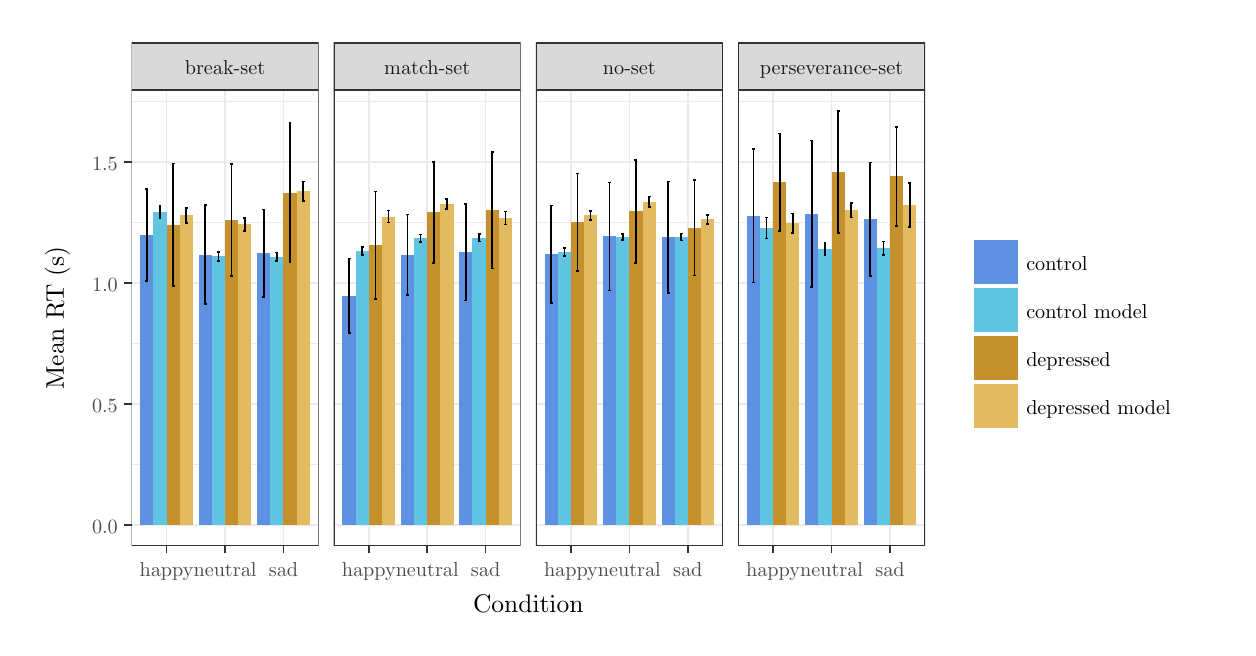
\begin{tikzpicture}[x=1pt,y=1pt]
\definecolor{fillColor}{RGB}{255,255,255}
\path[use as bounding box,fill=fillColor,fill opacity=0.00] (0,0) rectangle (433.62,216.81);
\begin{scope}
\path[clip] (  0.00,  0.00) rectangle (433.62,216.81);
\definecolor{drawColor}{RGB}{255,255,255}
\definecolor{fillColor}{RGB}{255,255,255}

\path[draw=drawColor,line width= 0.6pt,line join=round,line cap=round,fill=fillColor] (  0.00,  0.00) rectangle (433.62,216.81);
\end{scope}
\begin{scope}
\path[clip] ( 37.53, 29.59) rectangle (105.09,194.25);
\definecolor{fillColor}{RGB}{255,255,255}

\path[fill=fillColor] ( 37.53, 29.59) rectangle (105.09,194.25);
\definecolor{drawColor}{gray}{0.92}

\path[draw=drawColor,line width= 0.3pt,line join=round] ( 37.53, 58.93) --
	(105.09, 58.93);

\path[draw=drawColor,line width= 0.3pt,line join=round] ( 37.53,102.65) --
	(105.09,102.65);

\path[draw=drawColor,line width= 0.3pt,line join=round] ( 37.53,146.37) --
	(105.09,146.37);

\path[draw=drawColor,line width= 0.3pt,line join=round] ( 37.53,190.09) --
	(105.09,190.09);

\path[draw=drawColor,line width= 0.6pt,line join=round] ( 37.53, 37.07) --
	(105.09, 37.07);

\path[draw=drawColor,line width= 0.6pt,line join=round] ( 37.53, 80.79) --
	(105.09, 80.79);

\path[draw=drawColor,line width= 0.6pt,line join=round] ( 37.53,124.51) --
	(105.09,124.51);

\path[draw=drawColor,line width= 0.6pt,line join=round] ( 37.53,168.23) --
	(105.09,168.23);

\path[draw=drawColor,line width= 0.6pt,line join=round] ( 50.20, 29.59) --
	( 50.20,194.25);

\path[draw=drawColor,line width= 0.6pt,line join=round] ( 71.31, 29.59) --
	( 71.31,194.25);

\path[draw=drawColor,line width= 0.6pt,line join=round] ( 92.42, 29.59) --
	( 92.42,194.25);
\definecolor{fillColor}{RGB}{226,186,95}

\path[fill=fillColor] ( 54.95, 37.07) rectangle ( 59.70,148.94);
\definecolor{fillColor}{RGB}{196,145,45}

\path[fill=fillColor] ( 50.20, 37.07) rectangle ( 54.95,145.58);
\definecolor{fillColor}{RGB}{95,197,226}

\path[fill=fillColor] ( 45.45, 37.07) rectangle ( 50.20,150.14);
\definecolor{fillColor}{RGB}{95,145,226}

\path[fill=fillColor] ( 40.70, 37.07) rectangle ( 45.45,141.91);
\definecolor{fillColor}{RGB}{226,186,95}

\path[fill=fillColor] ( 76.06, 37.07) rectangle ( 80.81,145.70);
\definecolor{fillColor}{RGB}{196,145,45}

\path[fill=fillColor] ( 71.31, 37.07) rectangle ( 76.06,147.33);
\definecolor{fillColor}{RGB}{95,197,226}

\path[fill=fillColor] ( 66.56, 37.07) rectangle ( 71.31,134.13);
\definecolor{fillColor}{RGB}{95,145,226}

\path[fill=fillColor] ( 61.81, 37.07) rectangle ( 66.56,134.83);
\definecolor{fillColor}{RGB}{226,186,95}

\path[fill=fillColor] ( 97.17, 37.07) rectangle (101.92,157.69);
\definecolor{fillColor}{RGB}{196,145,45}

\path[fill=fillColor] ( 92.42, 37.07) rectangle ( 97.17,157.21);
\definecolor{fillColor}{RGB}{95,197,226}

\path[fill=fillColor] ( 87.67, 37.07) rectangle ( 92.42,134.05);
\definecolor{fillColor}{RGB}{95,145,226}

\path[fill=fillColor] ( 82.92, 37.07) rectangle ( 87.67,135.26);
\definecolor{drawColor}{RGB}{0,0,0}

\path[draw=drawColor,line width= 0.6pt,line join=round] ( 56.80,151.57) --
	( 57.85,151.57);

\path[draw=drawColor,line width= 0.6pt,line join=round] ( 57.32,151.57) --
	( 57.32,146.30);

\path[draw=drawColor,line width= 0.6pt,line join=round] ( 56.80,146.30) --
	( 57.85,146.30);

\path[draw=drawColor,line width= 0.6pt,line join=round] ( 52.05,167.70) --
	( 53.10,167.70);

\path[draw=drawColor,line width= 0.6pt,line join=round] ( 52.57,167.70) --
	( 52.57,123.46);

\path[draw=drawColor,line width= 0.6pt,line join=round] ( 52.05,123.46) --
	( 53.10,123.46);

\path[draw=drawColor,line width= 0.6pt,line join=round] ( 47.30,152.29) --
	( 48.35,152.29);

\path[draw=drawColor,line width= 0.6pt,line join=round] ( 47.82,152.29) --
	( 47.82,147.98);

\path[draw=drawColor,line width= 0.6pt,line join=round] ( 47.30,147.98) --
	( 48.35,147.98);

\path[draw=drawColor,line width= 0.6pt,line join=round] ( 42.55,158.43) --
	( 43.60,158.43);

\path[draw=drawColor,line width= 0.6pt,line join=round] ( 43.07,158.43) --
	( 43.07,125.38);

\path[draw=drawColor,line width= 0.6pt,line join=round] ( 42.55,125.38) --
	( 43.60,125.38);

\path[draw=drawColor,line width= 0.6pt,line join=round] ( 77.91,148.13) --
	( 78.96,148.13);

\path[draw=drawColor,line width= 0.6pt,line join=round] ( 78.44,148.13) --
	( 78.44,143.27);

\path[draw=drawColor,line width= 0.6pt,line join=round] ( 77.91,143.27) --
	( 78.96,143.27);

\path[draw=drawColor,line width= 0.6pt,line join=round] ( 73.16,167.62) --
	( 74.21,167.62);

\path[draw=drawColor,line width= 0.6pt,line join=round] ( 73.69,167.62) --
	( 73.69,127.04);

\path[draw=drawColor,line width= 0.6pt,line join=round] ( 73.16,127.04) --
	( 74.21,127.04);

\path[draw=drawColor,line width= 0.6pt,line join=round] ( 68.41,135.71) --
	( 69.46,135.71);

\path[draw=drawColor,line width= 0.6pt,line join=round] ( 68.94,135.71) --
	( 68.94,132.56);

\path[draw=drawColor,line width= 0.6pt,line join=round] ( 68.41,132.56) --
	( 69.46,132.56);

\path[draw=drawColor,line width= 0.6pt,line join=round] ( 63.66,152.75) --
	( 64.71,152.75);

\path[draw=drawColor,line width= 0.6pt,line join=round] ( 64.19,152.75) --
	( 64.19,116.90);

\path[draw=drawColor,line width= 0.6pt,line join=round] ( 63.66,116.90) --
	( 64.71,116.90);

\path[draw=drawColor,line width= 0.6pt,line join=round] ( 99.02,161.19) --
	(100.07,161.19);

\path[draw=drawColor,line width= 0.6pt,line join=round] ( 99.55,161.19) --
	( 99.55,154.18);

\path[draw=drawColor,line width= 0.6pt,line join=round] ( 99.02,154.18) --
	(100.07,154.18);

\path[draw=drawColor,line width= 0.6pt,line join=round] ( 94.27,182.39) --
	( 95.32,182.39);

\path[draw=drawColor,line width= 0.6pt,line join=round] ( 94.80,182.39) --
	( 94.80,132.03);

\path[draw=drawColor,line width= 0.6pt,line join=round] ( 94.27,132.03) --
	( 95.32,132.03);

\path[draw=drawColor,line width= 0.6pt,line join=round] ( 89.52,135.60) --
	( 90.57,135.60);

\path[draw=drawColor,line width= 0.6pt,line join=round] ( 90.05,135.60) --
	( 90.05,132.51);

\path[draw=drawColor,line width= 0.6pt,line join=round] ( 89.52,132.51) --
	( 90.57,132.51);

\path[draw=drawColor,line width= 0.6pt,line join=round] ( 84.77,151.09) --
	( 85.82,151.09);

\path[draw=drawColor,line width= 0.6pt,line join=round] ( 85.30,151.09) --
	( 85.30,119.44);

\path[draw=drawColor,line width= 0.6pt,line join=round] ( 84.77,119.44) --
	( 85.82,119.44);
\definecolor{drawColor}{gray}{0.20}

\path[draw=drawColor,line width= 0.6pt,line join=round,line cap=round] ( 37.53, 29.59) rectangle (105.09,194.25);
\end{scope}
\begin{scope}
\path[clip] (110.59, 29.59) rectangle (178.14,194.25);
\definecolor{fillColor}{RGB}{255,255,255}

\path[fill=fillColor] (110.59, 29.59) rectangle (178.14,194.25);
\definecolor{drawColor}{gray}{0.92}

\path[draw=drawColor,line width= 0.3pt,line join=round] (110.59, 58.93) --
	(178.14, 58.93);

\path[draw=drawColor,line width= 0.3pt,line join=round] (110.59,102.65) --
	(178.14,102.65);

\path[draw=drawColor,line width= 0.3pt,line join=round] (110.59,146.37) --
	(178.14,146.37);

\path[draw=drawColor,line width= 0.3pt,line join=round] (110.59,190.09) --
	(178.14,190.09);

\path[draw=drawColor,line width= 0.6pt,line join=round] (110.59, 37.07) --
	(178.14, 37.07);

\path[draw=drawColor,line width= 0.6pt,line join=round] (110.59, 80.79) --
	(178.14, 80.79);

\path[draw=drawColor,line width= 0.6pt,line join=round] (110.59,124.51) --
	(178.14,124.51);

\path[draw=drawColor,line width= 0.6pt,line join=round] (110.59,168.23) --
	(178.14,168.23);

\path[draw=drawColor,line width= 0.6pt,line join=round] (123.25, 29.59) --
	(123.25,194.25);

\path[draw=drawColor,line width= 0.6pt,line join=round] (144.37, 29.59) --
	(144.37,194.25);

\path[draw=drawColor,line width= 0.6pt,line join=round] (165.48, 29.59) --
	(165.48,194.25);
\definecolor{fillColor}{RGB}{226,186,95}

\path[fill=fillColor] (128.00, 37.07) rectangle (132.75,148.54);
\definecolor{fillColor}{RGB}{196,145,45}

\path[fill=fillColor] (123.25, 37.07) rectangle (128.00,138.15);
\definecolor{fillColor}{RGB}{95,197,226}

\path[fill=fillColor] (118.50, 37.07) rectangle (123.25,136.06);
\definecolor{fillColor}{RGB}{95,145,226}

\path[fill=fillColor] (113.75, 37.07) rectangle (118.50,119.96);
\definecolor{fillColor}{RGB}{226,186,95}

\path[fill=fillColor] (149.12, 37.07) rectangle (153.87,153.12);
\definecolor{fillColor}{RGB}{196,145,45}

\path[fill=fillColor] (144.37, 37.07) rectangle (149.12,150.04);
\definecolor{fillColor}{RGB}{95,197,226}

\path[fill=fillColor] (139.62, 37.07) rectangle (144.37,140.78);
\definecolor{fillColor}{RGB}{95,145,226}

\path[fill=fillColor] (134.87, 37.07) rectangle (139.62,134.74);
\definecolor{fillColor}{RGB}{226,186,95}

\path[fill=fillColor] (170.23, 37.07) rectangle (174.98,148.00);
\definecolor{fillColor}{RGB}{196,145,45}

\path[fill=fillColor] (165.48, 37.07) rectangle (170.23,150.92);
\definecolor{fillColor}{RGB}{95,197,226}

\path[fill=fillColor] (160.73, 37.07) rectangle (165.48,140.83);
\definecolor{fillColor}{RGB}{95,145,226}

\path[fill=fillColor] (155.98, 37.07) rectangle (160.73,135.61);
\definecolor{drawColor}{RGB}{0,0,0}

\path[draw=drawColor,line width= 0.6pt,line join=round] (129.85,150.70) --
	(130.91,150.70);

\path[draw=drawColor,line width= 0.6pt,line join=round] (130.38,150.70) --
	(130.38,146.39);

\path[draw=drawColor,line width= 0.6pt,line join=round] (129.85,146.39) --
	(130.91,146.39);

\path[draw=drawColor,line width= 0.6pt,line join=round] (125.10,157.56) --
	(126.16,157.56);

\path[draw=drawColor,line width= 0.6pt,line join=round] (125.63,157.56) --
	(125.63,118.74);

\path[draw=drawColor,line width= 0.6pt,line join=round] (125.10,118.74) --
	(126.16,118.74);

\path[draw=drawColor,line width= 0.6pt,line join=round] (120.35,137.44) --
	(121.41,137.44);

\path[draw=drawColor,line width= 0.6pt,line join=round] (120.88,137.44) --
	(120.88,134.69);

\path[draw=drawColor,line width= 0.6pt,line join=round] (120.35,134.69) --
	(121.41,134.69);

\path[draw=drawColor,line width= 0.6pt,line join=round] (115.60,133.43) --
	(116.66,133.43);

\path[draw=drawColor,line width= 0.6pt,line join=round] (116.13,133.43) --
	(116.13,106.50);

\path[draw=drawColor,line width= 0.6pt,line join=round] (115.60,106.50) --
	(116.66,106.50);

\path[draw=drawColor,line width= 0.6pt,line join=round] (150.96,154.86) --
	(152.02,154.86);

\path[draw=drawColor,line width= 0.6pt,line join=round] (151.49,154.86) --
	(151.49,151.38);

\path[draw=drawColor,line width= 0.6pt,line join=round] (150.96,151.38) --
	(152.02,151.38);

\path[draw=drawColor,line width= 0.6pt,line join=round] (146.21,168.32) --
	(147.27,168.32);

\path[draw=drawColor,line width= 0.6pt,line join=round] (146.74,168.32) --
	(146.74,131.77);

\path[draw=drawColor,line width= 0.6pt,line join=round] (146.21,131.77) --
	(147.27,131.77);

\path[draw=drawColor,line width= 0.6pt,line join=round] (141.46,142.12) --
	(142.52,142.12);

\path[draw=drawColor,line width= 0.6pt,line join=round] (141.99,142.12) --
	(141.99,139.44);

\path[draw=drawColor,line width= 0.6pt,line join=round] (141.46,139.44) --
	(142.52,139.44);

\path[draw=drawColor,line width= 0.6pt,line join=round] (136.71,149.34) --
	(137.77,149.34);

\path[draw=drawColor,line width= 0.6pt,line join=round] (137.24,149.34) --
	(137.24,120.14);

\path[draw=drawColor,line width= 0.6pt,line join=round] (136.71,120.14) --
	(137.77,120.14);

\path[draw=drawColor,line width= 0.6pt,line join=round] (172.07,150.38) --
	(173.13,150.38);

\path[draw=drawColor,line width= 0.6pt,line join=round] (172.60,150.38) --
	(172.60,145.63);

\path[draw=drawColor,line width= 0.6pt,line join=round] (172.07,145.63) --
	(173.13,145.63);

\path[draw=drawColor,line width= 0.6pt,line join=round] (167.32,171.99) --
	(168.38,171.99);

\path[draw=drawColor,line width= 0.6pt,line join=round] (167.85,171.99) --
	(167.85,129.84);

\path[draw=drawColor,line width= 0.6pt,line join=round] (167.32,129.84) --
	(168.38,129.84);

\path[draw=drawColor,line width= 0.6pt,line join=round] (162.57,142.15) --
	(163.63,142.15);

\path[draw=drawColor,line width= 0.6pt,line join=round] (163.10,142.15) --
	(163.10,139.51);

\path[draw=drawColor,line width= 0.6pt,line join=round] (162.57,139.51) --
	(163.63,139.51);

\path[draw=drawColor,line width= 0.6pt,line join=round] (157.82,153.01) --
	(158.88,153.01);

\path[draw=drawColor,line width= 0.6pt,line join=round] (158.35,153.01) --
	(158.35,118.21);

\path[draw=drawColor,line width= 0.6pt,line join=round] (157.82,118.21) --
	(158.88,118.21);
\definecolor{drawColor}{gray}{0.20}

\path[draw=drawColor,line width= 0.6pt,line join=round,line cap=round] (110.59, 29.59) rectangle (178.14,194.25);
\end{scope}
\begin{scope}
\path[clip] (183.64, 29.59) rectangle (251.20,194.25);
\definecolor{fillColor}{RGB}{255,255,255}

\path[fill=fillColor] (183.64, 29.59) rectangle (251.20,194.25);
\definecolor{drawColor}{gray}{0.92}

\path[draw=drawColor,line width= 0.3pt,line join=round] (183.64, 58.93) --
	(251.20, 58.93);

\path[draw=drawColor,line width= 0.3pt,line join=round] (183.64,102.65) --
	(251.20,102.65);

\path[draw=drawColor,line width= 0.3pt,line join=round] (183.64,146.37) --
	(251.20,146.37);

\path[draw=drawColor,line width= 0.3pt,line join=round] (183.64,190.09) --
	(251.20,190.09);

\path[draw=drawColor,line width= 0.6pt,line join=round] (183.64, 37.07) --
	(251.20, 37.07);

\path[draw=drawColor,line width= 0.6pt,line join=round] (183.64, 80.79) --
	(251.20, 80.79);

\path[draw=drawColor,line width= 0.6pt,line join=round] (183.64,124.51) --
	(251.20,124.51);

\path[draw=drawColor,line width= 0.6pt,line join=round] (183.64,168.23) --
	(251.20,168.23);

\path[draw=drawColor,line width= 0.6pt,line join=round] (196.31, 29.59) --
	(196.31,194.25);

\path[draw=drawColor,line width= 0.6pt,line join=round] (217.42, 29.59) --
	(217.42,194.25);

\path[draw=drawColor,line width= 0.6pt,line join=round] (238.53, 29.59) --
	(238.53,194.25);
\definecolor{fillColor}{RGB}{226,186,95}

\path[fill=fillColor] (201.06, 37.07) rectangle (205.81,148.98);
\definecolor{fillColor}{RGB}{196,145,45}

\path[fill=fillColor] (196.31, 37.07) rectangle (201.06,146.46);
\definecolor{fillColor}{RGB}{95,197,226}

\path[fill=fillColor] (191.56, 37.07) rectangle (196.31,135.80);
\definecolor{fillColor}{RGB}{95,145,226}

\path[fill=fillColor] (186.81, 37.07) rectangle (191.56,134.91);
\definecolor{fillColor}{RGB}{226,186,95}

\path[fill=fillColor] (222.17, 37.07) rectangle (226.92,153.91);
\definecolor{fillColor}{RGB}{196,145,45}

\path[fill=fillColor] (217.42, 37.07) rectangle (222.17,150.39);
\definecolor{fillColor}{RGB}{95,197,226}

\path[fill=fillColor] (212.67, 37.07) rectangle (217.42,141.14);
\definecolor{fillColor}{RGB}{95,145,226}

\path[fill=fillColor] (207.92, 37.07) rectangle (212.67,141.38);
\definecolor{fillColor}{RGB}{226,186,95}

\path[fill=fillColor] (243.28, 37.07) rectangle (248.03,147.55);
\definecolor{fillColor}{RGB}{196,145,45}

\path[fill=fillColor] (238.53, 37.07) rectangle (243.28,144.44);
\definecolor{fillColor}{RGB}{95,197,226}

\path[fill=fillColor] (233.78, 37.07) rectangle (238.53,141.18);
\definecolor{fillColor}{RGB}{95,145,226}

\path[fill=fillColor] (229.03, 37.07) rectangle (233.78,141.12);
\definecolor{drawColor}{RGB}{0,0,0}

\path[draw=drawColor,line width= 0.6pt,line join=round] (202.91,150.67) --
	(203.96,150.67);

\path[draw=drawColor,line width= 0.6pt,line join=round] (203.43,150.67) --
	(203.43,147.30);

\path[draw=drawColor,line width= 0.6pt,line join=round] (202.91,147.30) --
	(203.96,147.30);

\path[draw=drawColor,line width= 0.6pt,line join=round] (198.16,164.12) --
	(199.21,164.12);

\path[draw=drawColor,line width= 0.6pt,line join=round] (198.68,164.12) --
	(198.68,128.79);

\path[draw=drawColor,line width= 0.6pt,line join=round] (198.16,128.79) --
	(199.21,128.79);

\path[draw=drawColor,line width= 0.6pt,line join=round] (193.41,137.23) --
	(194.46,137.23);

\path[draw=drawColor,line width= 0.6pt,line join=round] (193.93,137.23) --
	(193.93,134.36);

\path[draw=drawColor,line width= 0.6pt,line join=round] (193.41,134.36) --
	(194.46,134.36);

\path[draw=drawColor,line width= 0.6pt,line join=round] (188.66,152.49) --
	(189.71,152.49);

\path[draw=drawColor,line width= 0.6pt,line join=round] (189.18,152.49) --
	(189.18,117.34);

\path[draw=drawColor,line width= 0.6pt,line join=round] (188.66,117.34) --
	(189.71,117.34);

\path[draw=drawColor,line width= 0.6pt,line join=round] (224.02,155.79) --
	(225.07,155.79);

\path[draw=drawColor,line width= 0.6pt,line join=round] (224.55,155.79) --
	(224.55,152.03);

\path[draw=drawColor,line width= 0.6pt,line join=round] (224.02,152.03) --
	(225.07,152.03);

\path[draw=drawColor,line width= 0.6pt,line join=round] (219.27,168.93) --
	(220.32,168.93);

\path[draw=drawColor,line width= 0.6pt,line join=round] (219.80,168.93) --
	(219.80,131.85);

\path[draw=drawColor,line width= 0.6pt,line join=round] (219.27,131.85) --
	(220.32,131.85);

\path[draw=drawColor,line width= 0.6pt,line join=round] (214.52,142.24) --
	(215.57,142.24);

\path[draw=drawColor,line width= 0.6pt,line join=round] (215.05,142.24) --
	(215.05,140.05);

\path[draw=drawColor,line width= 0.6pt,line join=round] (214.52,140.05) --
	(215.57,140.05);

\path[draw=drawColor,line width= 0.6pt,line join=round] (209.77,160.88) --
	(210.82,160.88);

\path[draw=drawColor,line width= 0.6pt,line join=round] (210.30,160.88) --
	(210.30,121.89);

\path[draw=drawColor,line width= 0.6pt,line join=round] (209.77,121.89) --
	(210.82,121.89);

\path[draw=drawColor,line width= 0.6pt,line join=round] (245.13,149.19) --
	(246.18,149.19);

\path[draw=drawColor,line width= 0.6pt,line join=round] (245.66,149.19) --
	(245.66,145.92);

\path[draw=drawColor,line width= 0.6pt,line join=round] (245.13,145.92) --
	(246.18,145.92);

\path[draw=drawColor,line width= 0.6pt,line join=round] (240.38,161.67) --
	(241.43,161.67);

\path[draw=drawColor,line width= 0.6pt,line join=round] (240.91,161.67) --
	(240.91,127.22);

\path[draw=drawColor,line width= 0.6pt,line join=round] (240.38,127.22) --
	(241.43,127.22);

\path[draw=drawColor,line width= 0.6pt,line join=round] (235.63,142.44) --
	(236.68,142.44);

\path[draw=drawColor,line width= 0.6pt,line join=round] (236.16,142.44) --
	(236.16,139.93);

\path[draw=drawColor,line width= 0.6pt,line join=round] (235.63,139.93) --
	(236.68,139.93);

\path[draw=drawColor,line width= 0.6pt,line join=round] (230.88,161.23) --
	(231.93,161.23);

\path[draw=drawColor,line width= 0.6pt,line join=round] (231.41,161.23) --
	(231.41,121.01);

\path[draw=drawColor,line width= 0.6pt,line join=round] (230.88,121.01) --
	(231.93,121.01);
\definecolor{drawColor}{gray}{0.20}

\path[draw=drawColor,line width= 0.6pt,line join=round,line cap=round] (183.64, 29.59) rectangle (251.20,194.25);
\end{scope}
\begin{scope}
\path[clip] (256.70, 29.59) rectangle (324.25,194.25);
\definecolor{fillColor}{RGB}{255,255,255}

\path[fill=fillColor] (256.70, 29.59) rectangle (324.25,194.25);
\definecolor{drawColor}{gray}{0.92}

\path[draw=drawColor,line width= 0.3pt,line join=round] (256.70, 58.93) --
	(324.25, 58.93);

\path[draw=drawColor,line width= 0.3pt,line join=round] (256.70,102.65) --
	(324.25,102.65);

\path[draw=drawColor,line width= 0.3pt,line join=round] (256.70,146.37) --
	(324.25,146.37);

\path[draw=drawColor,line width= 0.3pt,line join=round] (256.70,190.09) --
	(324.25,190.09);

\path[draw=drawColor,line width= 0.6pt,line join=round] (256.70, 37.07) --
	(324.25, 37.07);

\path[draw=drawColor,line width= 0.6pt,line join=round] (256.70, 80.79) --
	(324.25, 80.79);

\path[draw=drawColor,line width= 0.6pt,line join=round] (256.70,124.51) --
	(324.25,124.51);

\path[draw=drawColor,line width= 0.6pt,line join=round] (256.70,168.23) --
	(324.25,168.23);

\path[draw=drawColor,line width= 0.6pt,line join=round] (269.36, 29.59) --
	(269.36,194.25);

\path[draw=drawColor,line width= 0.6pt,line join=round] (290.48, 29.59) --
	(290.48,194.25);

\path[draw=drawColor,line width= 0.6pt,line join=round] (311.59, 29.59) --
	(311.59,194.25);
\definecolor{fillColor}{RGB}{226,186,95}

\path[fill=fillColor] (274.11, 37.07) rectangle (278.86,146.20);
\definecolor{fillColor}{RGB}{196,145,45}

\path[fill=fillColor] (269.36, 37.07) rectangle (274.11,160.97);
\definecolor{fillColor}{RGB}{95,197,226}

\path[fill=fillColor] (264.61, 37.07) rectangle (269.36,144.41);
\definecolor{fillColor}{RGB}{95,145,226}

\path[fill=fillColor] (259.86, 37.07) rectangle (264.61,148.82);
\definecolor{fillColor}{RGB}{226,186,95}

\path[fill=fillColor] (295.23, 37.07) rectangle (299.98,150.86);
\definecolor{fillColor}{RGB}{196,145,45}

\path[fill=fillColor] (290.48, 37.07) rectangle (295.23,164.73);
\definecolor{fillColor}{RGB}{95,197,226}

\path[fill=fillColor] (285.73, 37.07) rectangle (290.48,136.74);
\definecolor{fillColor}{RGB}{95,145,226}

\path[fill=fillColor] (280.98, 37.07) rectangle (285.73,149.52);
\definecolor{fillColor}{RGB}{226,186,95}

\path[fill=fillColor] (316.34, 37.07) rectangle (321.09,152.67);
\definecolor{fillColor}{RGB}{196,145,45}

\path[fill=fillColor] (311.59, 37.07) rectangle (316.34,163.07);
\definecolor{fillColor}{RGB}{95,197,226}

\path[fill=fillColor] (306.84, 37.07) rectangle (311.59,137.12);
\definecolor{fillColor}{RGB}{95,145,226}

\path[fill=fillColor] (302.09, 37.07) rectangle (306.84,147.51);
\definecolor{drawColor}{RGB}{0,0,0}

\path[draw=drawColor,line width= 0.6pt,line join=round] (275.96,149.71) --
	(277.02,149.71);

\path[draw=drawColor,line width= 0.6pt,line join=round] (276.49,149.71) --
	(276.49,142.70);

\path[draw=drawColor,line width= 0.6pt,line join=round] (275.96,142.70) --
	(277.02,142.70);

\path[draw=drawColor,line width= 0.6pt,line join=round] (271.21,178.55) --
	(272.27,178.55);

\path[draw=drawColor,line width= 0.6pt,line join=round] (271.74,178.55) --
	(271.74,143.40);

\path[draw=drawColor,line width= 0.6pt,line join=round] (271.21,143.40) --
	(272.27,143.40);

\path[draw=drawColor,line width= 0.6pt,line join=round] (266.46,148.16) --
	(267.52,148.16);

\path[draw=drawColor,line width= 0.6pt,line join=round] (266.99,148.16) --
	(266.99,140.66);

\path[draw=drawColor,line width= 0.6pt,line join=round] (266.46,140.66) --
	(267.52,140.66);

\path[draw=drawColor,line width= 0.6pt,line join=round] (261.71,172.95) --
	(262.77,172.95);

\path[draw=drawColor,line width= 0.6pt,line join=round] (262.24,172.95) --
	(262.24,124.68);

\path[draw=drawColor,line width= 0.6pt,line join=round] (261.71,124.68) --
	(262.77,124.68);

\path[draw=drawColor,line width= 0.6pt,line join=round] (297.07,153.44) --
	(298.13,153.44);

\path[draw=drawColor,line width= 0.6pt,line join=round] (297.60,153.44) --
	(297.60,148.27);

\path[draw=drawColor,line width= 0.6pt,line join=round] (297.07,148.27) --
	(298.13,148.27);

\path[draw=drawColor,line width= 0.6pt,line join=round] (292.32,186.76) --
	(293.38,186.76);

\path[draw=drawColor,line width= 0.6pt,line join=round] (292.85,186.76) --
	(292.85,142.70);

\path[draw=drawColor,line width= 0.6pt,line join=round] (292.32,142.70) --
	(293.38,142.70);

\path[draw=drawColor,line width= 0.6pt,line join=round] (287.57,138.99) --
	(288.63,138.99);

\path[draw=drawColor,line width= 0.6pt,line join=round] (288.10,138.99) --
	(288.10,134.49);

\path[draw=drawColor,line width= 0.6pt,line join=round] (287.57,134.49) --
	(288.63,134.49);

\path[draw=drawColor,line width= 0.6pt,line join=round] (282.82,176.01) --
	(283.88,176.01);

\path[draw=drawColor,line width= 0.6pt,line join=round] (283.35,176.01) --
	(283.35,123.02);

\path[draw=drawColor,line width= 0.6pt,line join=round] (282.82,123.02) --
	(283.88,123.02);

\path[draw=drawColor,line width= 0.6pt,line join=round] (318.18,160.65) --
	(319.24,160.65);

\path[draw=drawColor,line width= 0.6pt,line join=round] (318.71,160.65) --
	(318.71,144.69);

\path[draw=drawColor,line width= 0.6pt,line join=round] (318.18,144.69) --
	(319.24,144.69);

\path[draw=drawColor,line width= 0.6pt,line join=round] (313.43,180.99) --
	(314.49,180.99);

\path[draw=drawColor,line width= 0.6pt,line join=round] (313.96,180.99) --
	(313.96,145.14);

\path[draw=drawColor,line width= 0.6pt,line join=round] (313.43,145.14) --
	(314.49,145.14);

\path[draw=drawColor,line width= 0.6pt,line join=round] (308.68,139.49) --
	(309.74,139.49);

\path[draw=drawColor,line width= 0.6pt,line join=round] (309.21,139.49) --
	(309.21,134.74);

\path[draw=drawColor,line width= 0.6pt,line join=round] (308.68,134.74) --
	(309.74,134.74);

\path[draw=drawColor,line width= 0.6pt,line join=round] (303.93,168.05) --
	(304.99,168.05);

\path[draw=drawColor,line width= 0.6pt,line join=round] (304.46,168.05) --
	(304.46,126.96);

\path[draw=drawColor,line width= 0.6pt,line join=round] (303.93,126.96) --
	(304.99,126.96);
\definecolor{drawColor}{gray}{0.20}

\path[draw=drawColor,line width= 0.6pt,line join=round,line cap=round] (256.70, 29.59) rectangle (324.25,194.25);
\end{scope}
\begin{scope}
\path[clip] ( 37.53,194.25) rectangle (105.09,211.31);
\definecolor{drawColor}{gray}{0.20}
\definecolor{fillColor}{gray}{0.85}

\path[draw=drawColor,line width= 0.6pt,line join=round,line cap=round,fill=fillColor] ( 37.53,194.25) rectangle (105.09,211.31);
\definecolor{drawColor}{gray}{0.10}

\node[text=drawColor,anchor=base,inner sep=0pt, outer sep=0pt, scale=  0.73] at ( 71.31,199.75) {break-set};
\end{scope}
\begin{scope}
\path[clip] (110.59,194.25) rectangle (178.14,211.31);
\definecolor{drawColor}{gray}{0.20}
\definecolor{fillColor}{gray}{0.85}

\path[draw=drawColor,line width= 0.6pt,line join=round,line cap=round,fill=fillColor] (110.59,194.25) rectangle (178.14,211.31);
\definecolor{drawColor}{gray}{0.10}

\node[text=drawColor,anchor=base,inner sep=0pt, outer sep=0pt, scale=  0.73] at (144.37,199.75) {match-set};
\end{scope}
\begin{scope}
\path[clip] (183.64,194.25) rectangle (251.20,211.31);
\definecolor{drawColor}{gray}{0.20}
\definecolor{fillColor}{gray}{0.85}

\path[draw=drawColor,line width= 0.6pt,line join=round,line cap=round,fill=fillColor] (183.64,194.25) rectangle (251.20,211.31);
\definecolor{drawColor}{gray}{0.10}

\node[text=drawColor,anchor=base,inner sep=0pt, outer sep=0pt, scale=  0.73] at (217.42,199.75) {no-set};
\end{scope}
\begin{scope}
\path[clip] (256.70,194.25) rectangle (324.25,211.31);
\definecolor{drawColor}{gray}{0.20}
\definecolor{fillColor}{gray}{0.85}

\path[draw=drawColor,line width= 0.6pt,line join=round,line cap=round,fill=fillColor] (256.70,194.25) rectangle (324.25,211.31);
\definecolor{drawColor}{gray}{0.10}

\node[text=drawColor,anchor=base,inner sep=0pt, outer sep=0pt, scale=  0.73] at (290.48,199.75) {perseverance-set};
\end{scope}
\begin{scope}
\path[clip] (  0.00,  0.00) rectangle (433.62,216.81);
\definecolor{drawColor}{gray}{0.20}

\path[draw=drawColor,line width= 0.6pt,line join=round] ( 50.20, 26.84) --
	( 50.20, 29.59);

\path[draw=drawColor,line width= 0.6pt,line join=round] ( 71.31, 26.84) --
	( 71.31, 29.59);

\path[draw=drawColor,line width= 0.6pt,line join=round] ( 92.42, 26.84) --
	( 92.42, 29.59);
\end{scope}
\begin{scope}
\path[clip] (  0.00,  0.00) rectangle (433.62,216.81);
\definecolor{drawColor}{gray}{0.30}

\node[text=drawColor,anchor=base,inner sep=0pt, outer sep=0pt, scale=  0.73] at ( 50.20, 18.58) {happy};

\node[text=drawColor,anchor=base,inner sep=0pt, outer sep=0pt, scale=  0.73] at ( 71.31, 18.58) {neutral};

\node[text=drawColor,anchor=base,inner sep=0pt, outer sep=0pt, scale=  0.73] at ( 92.42, 18.58) {sad};
\end{scope}
\begin{scope}
\path[clip] (  0.00,  0.00) rectangle (433.62,216.81);
\definecolor{drawColor}{gray}{0.20}

\path[draw=drawColor,line width= 0.6pt,line join=round] (123.25, 26.84) --
	(123.25, 29.59);

\path[draw=drawColor,line width= 0.6pt,line join=round] (144.37, 26.84) --
	(144.37, 29.59);

\path[draw=drawColor,line width= 0.6pt,line join=round] (165.48, 26.84) --
	(165.48, 29.59);
\end{scope}
\begin{scope}
\path[clip] (  0.00,  0.00) rectangle (433.62,216.81);
\definecolor{drawColor}{gray}{0.30}

\node[text=drawColor,anchor=base,inner sep=0pt, outer sep=0pt, scale=  0.73] at (123.25, 18.58) {happy};

\node[text=drawColor,anchor=base,inner sep=0pt, outer sep=0pt, scale=  0.73] at (144.37, 18.58) {neutral};

\node[text=drawColor,anchor=base,inner sep=0pt, outer sep=0pt, scale=  0.73] at (165.48, 18.58) {sad};
\end{scope}
\begin{scope}
\path[clip] (  0.00,  0.00) rectangle (433.62,216.81);
\definecolor{drawColor}{gray}{0.20}

\path[draw=drawColor,line width= 0.6pt,line join=round] (196.31, 26.84) --
	(196.31, 29.59);

\path[draw=drawColor,line width= 0.6pt,line join=round] (217.42, 26.84) --
	(217.42, 29.59);

\path[draw=drawColor,line width= 0.6pt,line join=round] (238.53, 26.84) --
	(238.53, 29.59);
\end{scope}
\begin{scope}
\path[clip] (  0.00,  0.00) rectangle (433.62,216.81);
\definecolor{drawColor}{gray}{0.30}

\node[text=drawColor,anchor=base,inner sep=0pt, outer sep=0pt, scale=  0.73] at (196.31, 18.58) {happy};

\node[text=drawColor,anchor=base,inner sep=0pt, outer sep=0pt, scale=  0.73] at (217.42, 18.58) {neutral};

\node[text=drawColor,anchor=base,inner sep=0pt, outer sep=0pt, scale=  0.73] at (238.53, 18.58) {sad};
\end{scope}
\begin{scope}
\path[clip] (  0.00,  0.00) rectangle (433.62,216.81);
\definecolor{drawColor}{gray}{0.20}

\path[draw=drawColor,line width= 0.6pt,line join=round] (269.36, 26.84) --
	(269.36, 29.59);

\path[draw=drawColor,line width= 0.6pt,line join=round] (290.48, 26.84) --
	(290.48, 29.59);

\path[draw=drawColor,line width= 0.6pt,line join=round] (311.59, 26.84) --
	(311.59, 29.59);
\end{scope}
\begin{scope}
\path[clip] (  0.00,  0.00) rectangle (433.62,216.81);
\definecolor{drawColor}{gray}{0.30}

\node[text=drawColor,anchor=base,inner sep=0pt, outer sep=0pt, scale=  0.73] at (269.36, 18.58) {happy};

\node[text=drawColor,anchor=base,inner sep=0pt, outer sep=0pt, scale=  0.73] at (290.48, 18.58) {neutral};

\node[text=drawColor,anchor=base,inner sep=0pt, outer sep=0pt, scale=  0.73] at (311.59, 18.58) {sad};
\end{scope}
\begin{scope}
\path[clip] (  0.00,  0.00) rectangle (433.62,216.81);
\definecolor{drawColor}{gray}{0.30}

\node[text=drawColor,anchor=base east,inner sep=0pt, outer sep=0pt, scale=  0.73] at ( 32.58, 34.04) {0.0};

\node[text=drawColor,anchor=base east,inner sep=0pt, outer sep=0pt, scale=  0.73] at ( 32.58, 77.76) {0.5};

\node[text=drawColor,anchor=base east,inner sep=0pt, outer sep=0pt, scale=  0.73] at ( 32.58,121.48) {1.0};

\node[text=drawColor,anchor=base east,inner sep=0pt, outer sep=0pt, scale=  0.73] at ( 32.58,165.20) {1.5};
\end{scope}
\begin{scope}
\path[clip] (  0.00,  0.00) rectangle (433.62,216.81);
\definecolor{drawColor}{gray}{0.20}

\path[draw=drawColor,line width= 0.6pt,line join=round] ( 34.78, 37.07) --
	( 37.53, 37.07);

\path[draw=drawColor,line width= 0.6pt,line join=round] ( 34.78, 80.79) --
	( 37.53, 80.79);

\path[draw=drawColor,line width= 0.6pt,line join=round] ( 34.78,124.51) --
	( 37.53,124.51);

\path[draw=drawColor,line width= 0.6pt,line join=round] ( 34.78,168.23) --
	( 37.53,168.23);
\end{scope}
\begin{scope}
\path[clip] (  0.00,  0.00) rectangle (433.62,216.81);
\definecolor{drawColor}{RGB}{0,0,0}

\node[text=drawColor,anchor=base,inner sep=0pt, outer sep=0pt, scale=  0.92] at (180.89,  5.50) {Condition};
\end{scope}
\begin{scope}
\path[clip] (  0.00,  0.00) rectangle (433.62,216.81);
\definecolor{drawColor}{RGB}{0,0,0}

\node[text=drawColor,rotate= 90.00,anchor=base,inner sep=0pt, outer sep=0pt, scale=  0.92] at ( 13.08,111.92) {Mean RT (s)};
\end{scope}
\begin{scope}
\path[clip] (  0.00,  0.00) rectangle (433.62,216.81);
\definecolor{fillColor}{RGB}{255,255,255}

\path[fill=fillColor] (335.63, 65.58) rectangle (428.12,158.25);
\end{scope}
\begin{scope}
\path[clip] (  0.00,  0.00) rectangle (433.62,216.81);
\definecolor{fillColor}{RGB}{255,255,255}

\path[fill=fillColor] (341.32,123.31) rectangle (358.67,140.65);
\end{scope}
\begin{scope}
\path[clip] (  0.00,  0.00) rectangle (433.62,216.81);
\definecolor{fillColor}{RGB}{95,145,226}

\path[fill=fillColor] (342.04,124.02) rectangle (357.96,139.94);
\end{scope}
\begin{scope}
\path[clip] (  0.00,  0.00) rectangle (433.62,216.81);
\definecolor{fillColor}{RGB}{255,255,255}

\path[fill=fillColor] (341.32,105.96) rectangle (358.67,123.31);
\end{scope}
\begin{scope}
\path[clip] (  0.00,  0.00) rectangle (433.62,216.81);
\definecolor{fillColor}{RGB}{95,197,226}

\path[fill=fillColor] (342.04,106.67) rectangle (357.96,122.60);
\end{scope}
\begin{scope}
\path[clip] (  0.00,  0.00) rectangle (433.62,216.81);
\definecolor{fillColor}{RGB}{255,255,255}

\path[fill=fillColor] (341.32, 88.62) rectangle (358.67,105.96);
\end{scope}
\begin{scope}
\path[clip] (  0.00,  0.00) rectangle (433.62,216.81);
\definecolor{fillColor}{RGB}{196,145,45}

\path[fill=fillColor] (342.04, 89.33) rectangle (357.96,105.25);
\end{scope}
\begin{scope}
\path[clip] (  0.00,  0.00) rectangle (433.62,216.81);
\definecolor{fillColor}{RGB}{255,255,255}

\path[fill=fillColor] (341.32, 71.27) rectangle (358.67, 88.62);
\end{scope}
\begin{scope}
\path[clip] (  0.00,  0.00) rectangle (433.62,216.81);
\definecolor{fillColor}{RGB}{226,186,95}

\path[fill=fillColor] (342.04, 71.98) rectangle (357.96, 87.91);
\end{scope}
\begin{scope}
\path[clip] (  0.00,  0.00) rectangle (433.62,216.81);
\definecolor{drawColor}{RGB}{0,0,0}

\node[text=drawColor,anchor=base west,inner sep=0pt, outer sep=0pt, scale=  0.73] at (360.84,128.95) {control};
\end{scope}
\begin{scope}
\path[clip] (  0.00,  0.00) rectangle (433.62,216.81);
\definecolor{drawColor}{RGB}{0,0,0}

\node[text=drawColor,anchor=base west,inner sep=0pt, outer sep=0pt, scale=  0.73] at (360.84,111.60) {control model};
\end{scope}
\begin{scope}
\path[clip] (  0.00,  0.00) rectangle (433.62,216.81);
\definecolor{drawColor}{RGB}{0,0,0}

\node[text=drawColor,anchor=base west,inner sep=0pt, outer sep=0pt, scale=  0.73] at (360.84, 94.26) {depressed};
\end{scope}
\begin{scope}
\path[clip] (  0.00,  0.00) rectangle (433.62,216.81);
\definecolor{drawColor}{RGB}{0,0,0}

\node[text=drawColor,anchor=base west,inner sep=0pt, outer sep=0pt, scale=  0.73] at (360.84, 76.91) {depressed model};
\end{scope}
\end{tikzpicture}
